\documentclass[11pt,a4paper]{article}
\usepackage[margin=25mm]{geometry}
\usepackage[T1]{fontenc}
\usepackage[utf8]{inputenc}
\usepackage{lmodern,microtype}
\usepackage{amsmath,amssymb,amsthm,mathtools}
\usepackage{booktabs,array}
\usepackage{xcolor,xurl}
\usepackage[colorlinks=true,linkcolor=black,citecolor=black,urlcolor=black,hypertexnames=false]{hyperref}
\usepackage{graphicx}
\setlength{\parindent}{1.2em}
\setlength{\parskip}{0.15em}
\setlength{\emergencystretch}{2em}
\numberwithin{equation}{section}
\newtheorem{theorem}{Theorem}[section]
\newtheorem{lemma}[theorem]{Lemma}
\newtheorem{proposition}[theorem]{Proposition}
\newtheorem{corollary}[theorem]{Corollary}
\theoremstyle{definition}
\newtheorem{problem}[theorem]{Open problem}
\theoremstyle{remark}
\newtheorem{remark}[theorem]{Remark}
\newcommand{\ii}{\mathrm{i}}
\newcommand{\one}{\mathbf{1}}
\newcommand{\spec}{\operatorname{spec}}
\newcommand{\Om}{\Omega}
\newcommand{\eps}{\varepsilon}
\newcommand{\tr}{\operatorname{tr}}
\newcommand{\Qw}{Q_{\mathrm{w}}}
\newcommand{\bw}{\beta_{\mathrm{w}}}
\newcommand{\aw}{\alpha_{\mathrm{w}}}
\newcommand{\lw}{\lambda_{\mathrm{w}}}

\title{How fast can a driven Markov network oscillate?\vspace{0.3em}\\
\large A four-state counterexample to the affine Karpelevich conjecture,\\
and the exact dimension at which it fails}
\author{Anonymous}
\date{27 October 2026\\[2pt]\small Version 1.0.0-candidate (unrefereed). DOI: \href{https://doi.org/10.5281/zenodo.23687327}{10.5281/zenodo.23687327}.\\
\small Code and data: \url{https://github.com/ipitchford/affinity-karpelevich-threshold}}

\begin{document}
\maketitle

\begin{abstract}
The eigenvalues of a continuous-time Markov rate matrix decide how fast
its probability distribution relaxes and how strongly it can oscillate.
For transition matrices of discrete-time chains, the exact set of
possible eigenvalues is a classical object, the Karpelevich region.
In 2025, Xu, Kolchinsky, Delvenne and Ito conjectured that the
eigenvalues of rate matrices fill a ``squashed'' copy of this region:
stretch it by the fastest escape rate, and flatten its imaginary
direction by a factor set by the strongest thermodynamic driving force
around any cycle (the largest cycle affinity per step). We show that
this conjecture is false. An explicit four-state network with integer
rates, about \(8.4\,k_{\mathrm B}T\) of driving around its strongest
cycle, has an eigenvalue outside the conjectured region; one integer
inequality proves it. For networks of at most three states the
conjectured containment is true, so four is the smallest failing size.
The mechanism is simple: adding weak ``resetting'' transitions of size
\(\eps\) moves the eigenvalues only by an amount proportional to
\(\eps\), but relaxes the affinity factor by an amount proportional to
\(\eps^{2/3}\), which is much larger. This gives counterexamples near a
whole boundary arc in four states, an explicit interval
\(0<\eps\le 1/100\), exactly certified counterexamples in five and six
states, and an asymptotic construction in every dimension \(n\ge4\).
All counterexamples use networks in which every pair of states is
connected; whether the conjecture holds for single-cycle networks, the
setting in which it was tested, remains open. The proved ellipse and
polygon bounds are unaffected.
\end{abstract}

\section{Introduction}
\label{sec:intro}

\subsection{Why the eigenvalue region matters}

A finite-state Markov jump process is described by a rate matrix
(generator) \(Q\). A nonreal eigenvalue \(\lambda\) of \(Q\) is a mode
that oscillates at angular frequency \(|\operatorname{Im}\lambda|\) and
decays at rate \(-\operatorname{Re}\lambda\). The ratio
\(|\operatorname{Im}\lambda|/|\operatorname{Re}\lambda|\) measures how
many coherent oscillations the mode completes before it decays. Such
modes underlie biochemical clocks and molecular motors, and their
coherence is limited by thermodynamics: a network at equilibrium has a
real spectrum, and oscillations require driving. Barato and Seifert
proposed a bound on coherence in terms of the driving force and the
cycle length \cite{barato2017}, later proved by Ohga, Ito and
Kolchinsky \cite{ohga2023}. Uhl and Seifert conjectured an ellipse that
contains the whole rescaled spectrum \cite{uhl2019}; Kolchinsky, Ohga
and Ito proved it for discrete multicyclic generators and added a
polygonal bound \cite{kolchinsky2026}. Bounds of this kind are also
used in reverse: from a measured relaxation spectrum one infers a
minimum dissipation.

The driving force is measured by cycle affinities. For a directed cycle
\(c\) of a network, the affinity \(F_c\) is the logarithm of the product
of forward rates divided by the product of backward rates. In
isothermal systems it is the entropy produced, in units of
\(k_{\mathrm B}\), each time the cycle is completed.

For discrete time the corresponding problem was solved long ago. The
Karpelevich region \(\Om_n\) is the set of all eigenvalues of all
\(n\times n\) stochastic matrices \cite{karpelevich1951,ito1997}. It is
a curvilinear star inside the unit disc whose boundary arcs meet the
unit circle at the roots of unity of order at most \(n\)
(Figure~\ref{fig:overview}).

\subsection{The conjecture and the answer}

Xu, Kolchinsky, Delvenne and Ito \cite[Supplement, Eq.~(S3)]{xu2025}
proposed the natural continuous-time analogue: the eigenvalues of rate
matrices fill an affine image of \(\Om_n\), shifted and stretched by the
largest escape rate \(\alpha\) and flattened vertically by the factor
\(\beta'=\tanh(\max_c F_c/(2|c|))\) (the precise statement is quoted
in Section~\ref{sec:setup}). Undoing this transformation, every
eigenvalue \(\lambda\) of \(Q\) should give a ``rescaled eigenvalue''
\begin{equation}
\zeta=1+\frac{\operatorname{Re}\lambda}{\alpha}
      +\ii\,\frac{\operatorname{Im}\lambda}{\alpha\beta'}
\label{eq:zeta_intro}
\end{equation}
inside \(\Om_n\). The conjecture was supported by sampling single-cycle
networks.

We show that this fails. Figure~\ref{fig:overview} shows the
four-state counterexample \(\Qw\) of Section~\ref{sec:witness}. Its
plain uniformised eigenvalue \(1+\lambda/\alpha\) lies inside
\(\Om_4\), as it must; its rescaled eigenvalue \(\zeta\) lies just
outside the curved left boundary arc, while still inside the proved
ellipse (disc) and polygon bounds.

\begin{figure}[t]
\centering
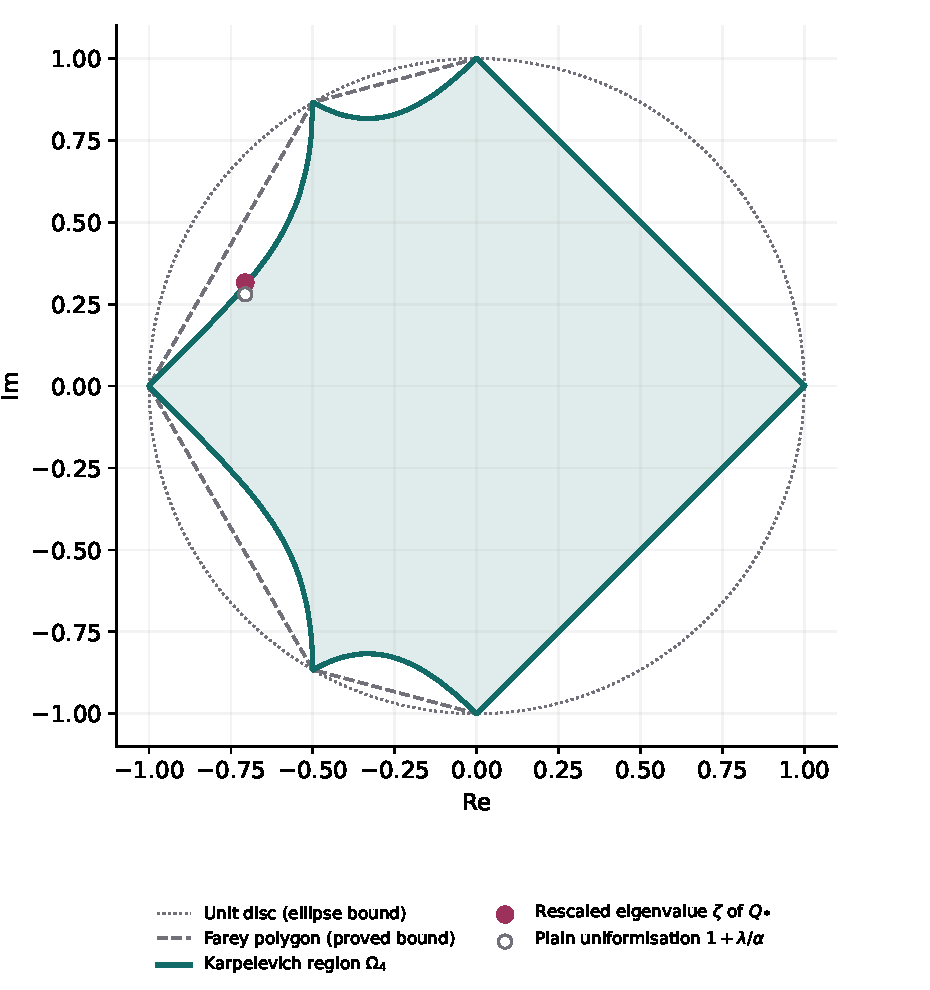
\includegraphics[width=0.72\textwidth]{region_overview.pdf}
\caption{The Karpelevich region \(\Om_4\) (shaded), the unit disc
(dotted; in these coordinates the proved affinity ellipse of
\cite{kolchinsky2026} becomes the unit disc), and the Farey polygon,
the convex hull of the roots of unity of order at most four (dashed;
the proved polygon bound of \cite[Theorem~5]{kolchinsky2026}). The
open circle is the plain uniformised eigenvalue \(1+\lw/\aw\) of the
witness \(\Qw\); the filled dot is its rescaled eigenvalue
\eqref{eq:zeta_intro}, which lies outside \(\Om_4\) but inside both
proved bounds. A magnified view is Figure~\ref{fig:geometry}.}
\label{fig:overview}
\end{figure}

\subsection{The idea in one paragraph}

Start from a stochastic matrix whose eigenvalue sits exactly on the
boundary of \(\Om_n\). Such matrices are known explicitly
\cite{johnson2017,kirkland2022}; some of their transitions are one-way.
Turn it into a rate matrix and add weak resetting: from every state,
jump with small rate proportional to \(\eps\) to a random state drawn
from the stationary distribution. Resetting of this kind shifts every
nonzero eigenvalue by the same amount, of order \(\eps\)
\cite{rose2018}. But it also creates reverse rates of order \(\eps\)
on the one-way edges. A triangle with two such edges then has affinity
about \(2\log(1/\eps)\), that is \(\frac23\log(1/\eps)\) per step, so
\(\beta'\) approaches \(1\) at rate \(\eps^{2/3}\). Dividing by
\(\beta'\) therefore pushes the rescaled eigenvalue outward by order
\(\eps^{2/3}\), while the eigenvalue itself has moved inward only by
order \(\eps\). For small \(\eps\) the outward push wins, and the
rescaled point leaves \(\Om_n\). In thermodynamic terms, the conjecture
spends the affinity budget through \(\tanh\), which saturates; a weak,
nearly irreversible back channel buys much affinity but little change
in the dynamics.

\subsection{Size of the effect, physical regime and scope}

The violation is a question of shape, not a large quantitative failure:
for \(\Qw\) the rescaled point exceeds the boundary by \(0.0087\) in
normalised units. The driving needed is moderate. The strongest cycle
of \(\Qw\) carries total affinity
\(\log(177853829/38529)\approx 8.44\), that is about
\(8.4\,k_{\mathrm B}T\), or \(2.8\,k_{\mathrm B}T\) per step, well
below the roughly \(20\,k_{\mathrm B}T\) of one ATP hydrolysis under
cellular conditions. The violating mode is poorly coherent:
\(|\operatorname{Im}\lambda|/|\operatorname{Re}\lambda|
=450\sqrt3/4745\approx0.16\). All constructions produce violations near
the left boundary arcs of \(\Om_n\), i.e.\ for strongly damped modes,
so they do not touch the high-coherence regime of biochemical clocks.

The practical consequence concerns inference. If the conjectured region
were used to infer a minimum affinity from the eigenvalue of \(\Qw\), it
would demand a per-step affinity \(M\approx3.075\), whereas the true
value is \(M\approx2.812\): an overestimate of about \(9\%\)
(Section~\ref{sec:discussion}). Table~\ref{tab:safe} summarises which
bounds remain safe.

\begin{table}[t]
\centering
\small
\begin{tabular}{@{}p{0.34\textwidth}p{0.2\textwidth}p{0.36\textwidth}@{}}
\toprule
Bound on the rescaled spectrum & Status & Source\\
\midrule
Sector (coherence) bound & proved & \cite{barato2017} (conjectured), \cite{ohga2023} (proof)\\
Affinity ellipse (unit disc in \(\zeta\)) & proved & \cite{uhl2019} (conjectured), \cite{kolchinsky2026}\\
Farey polygon & proved & \cite[Theorem~5]{kolchinsky2026}\\
Affine Karpelevich region (S3) & true for \(n\le3\); false for every \(n\ge4\) & this paper\\
Affine Karpelevich, single-cycle networks & open; no violation found numerically & Problem~\ref{prob:unicyclic}\\
\bottomrule
\end{tabular}
\caption{Which spectral bounds can be used for affinity inference.}
\label{tab:safe}
\end{table}

Scope matters. Every counterexample in this paper lives on the complete
graph: every pair of states is connected in both directions. The
``exact dimension threshold'' of the title refers to the universal
claim over all bidirectional networks of a given size: universal
containment holds for \(n\le3\) and fails for every \(n\ge4\). The
single-cycle (ring) networks that Xu et al.\ used as evidence are not
covered; we record them as an open problem with numerical evidence.

\subsection{Roadmap and what is new}

Section~\ref{sec:setup} quotes the conjecture and reduces it to a
containment (C). Section~\ref{sec:witness} gives the four-state witness
and its integer certificate. Section~\ref{sec:minimal} proves
containment for \(n\le3\). Sections~\ref{sec:family}
and~\ref{sec:uniform} explain the witness as one member of a resetting
family and give an explicit interval of counterexamples.
Section~\ref{sec:all_dimensions} extends the construction to every
\(n\ge4\) and gives exactly certified five- and six-state instances.
Section~\ref{sec:discussion} discusses consequences and open problems.

The boundary-realising matrices \cite{johnson2017,kirkland2022} and the
uniform spectral shift under resetting \cite{rose2018} are known. The
new contributions are the exact positive-rate witness, the
\(\eps\) versus \(\eps^{2/3}\) mechanism, the explicit interval, the
certified instances in five and six states, the extension to every
\(n\ge4\), and the proof of containment for \(n\le3\).

\section{The conjecture and the containment tested}
\label{sec:setup}

\subsection{Rate matrices and affinities}

We use the row convention. A rate matrix is a real matrix
\(Q=(q_{ij})_{i,j=1}^{n}\) with
\begin{equation}
q_{ij}\geq0\quad(i\ne j),\qquad
q_{ii}=-\sum_{j\ne i}q_{ij}.
\label{eq:generator}
\end{equation}
For \(n\geq2\) we assume that \(Q\) is irreducible and has bidirectional
support: \(q_{ij}>0\) if and only if \(q_{ji}>0\). The largest escape
rate
\begin{equation}
\alpha(Q)=\max_i(-q_{ii})>0
\end{equation}
sets the time unit: \(I+Q/\alpha\) is a stochastic matrix, so ordinary
uniformisation places \(1+\lambda/\alpha\) in \(\Om_n\) for every
\(\lambda\in\spec(Q)\).

For an oriented simple cycle \(c=(i_1,\ldots,i_m,i_1)\) in the support,
\begin{equation}
F_c=\log\prod_{k=1}^{m}
\frac{q_{i_k i_{k+1}}}{q_{i_{k+1}i_k}},\qquad
M(Q)=\max_c\frac{|F_c|}{|c|},\qquad
\beta(Q)=\tanh\frac{M(Q)}2,
\label{eq:affinity}
\end{equation}
with \(M=0\) if all affinities vanish. Thus \(M\) is the largest
affinity per step, and \(\beta\in[0,1)\) measures how far from
equilibrium the most driven cycle is. Two-cycles have zero affinity.
Allowing repeated closed walks gives the same maximum: a closed walk
decomposes into simple cycles, and its mean affinity cannot exceed the
largest simple-cycle mean. Reversing the orientation of \(c\) changes
the sign of \(F_c\); since the maximum in \cite{xu2025} runs over both
orientations, \(\max_c F_c/|c|=\max_c|F_c|/|c|\). The source uses the
column convention; transposing \(Q\) preserves the spectrum and \(M\).
If edge forces are defined with stationary fluxes
\(q_{ij}\pi_i/(q_{ji}\pi_j)\), the stationary factors cancel around
each cycle and give the same \(F_c\).

Our \(\beta\) is the parameter \(\beta'\) of \cite[Supplement]{xu2025}.
It differs from the parameter \(\beta\) of that paper's main theorem,
which uses the largest edge force \(\tanh(\max_e F_e/2)\).

\subsection{The conjecture, verbatim}

Let
\begin{equation}
\Om_n=\bigcup\{\spec(P):P\in\mathbb R^{n\times n},\ P\geq0,\ P\one=\one\}.
\label{eq:omega}
\end{equation}
Write \(R\) for a rate matrix in the column convention of
\cite{xu2025}, with \(\alpha=\max_i|R_{ii}|\) and
\(\beta'=\tanh(\max_c\{\mathcal F_c/(2n_c)\})\), where \(n_c\) is the
length of cycle \(c\). The supplement of \cite{xu2025} (Section~I.2)
states:

\begin{quote}
\emph{Conjecture.} The region \(\Om'_n\) of eigenvalues of the Markov
rate matrix \(R\) is the affine image of \(\Om_n\) under the
transformation:
\[
\Om'_n=\bigl\{\alpha(\operatorname{Re}z-1)+\ii\alpha\beta'\operatorname{Im}z
\;\big|\;z\in\Om_n\bigr\}.\qquad\text{(S3)}
\]
\end{quote}

Here \(\Om'_n\) is the set of eigenvalues of rate matrices of size
\(n\), and \(\alpha,\beta'\) are the values computed from \(R\). Two
readings are possible: for each \(R\), \(\spec(R)\) lies in the right
side; or the union of spectra over all rate matrices with given
\((\alpha,\beta')\) equals the right side. Both readings contain the
inclusion ``\(\subseteq\)'' for each individual matrix, and this is all
we use. Define
\begin{equation}
T_{\alpha,\beta}(z)
 =\alpha(\operatorname{Re}z-1)+\ii\alpha\beta\operatorname{Im}z .
\end{equation}

\begin{proposition}[(S3) implies (C)]
\label{prop:S3impliesC}
Under either reading, (S3) implies that every rate matrix \(Q\) of size
\(n\) satisfies
\begin{equation}
\spec(Q)\subseteq T_{\alpha(Q),\beta(Q)}(\Om_n).
\tag{C}\label{eq:conjecture}
\end{equation}
Hence any rate matrix violating \eqref{eq:conjecture} refutes (S3).
\end{proposition}

\begin{proof}
Let \(R=Q^{\mathsf T}\). Then \(\spec(R)=\spec(Q)\), \(\alpha\) is
unchanged, and \(\beta'(R)=\beta(Q)\) by the orientation remark above.
Each eigenvalue of \(R\) belongs to \(\Om'_n\) under either reading, and
(S3) says \(\Om'_n=T_{\alpha,\beta'}(\Om_n)\).
\end{proof}

Refuting \eqref{eq:conjecture} therefore needs no interpretation of
which boundary points are attained. When \(\beta>0\),
\eqref{eq:conjecture} says that every eigenvalue has rescaled
coordinate
\begin{equation}
\zeta_Q(\lambda)
 =1+\frac{\operatorname{Re}\lambda}{\alpha}
  +\ii\frac{\operatorname{Im}\lambda}{\alpha\beta}
 \in\Om_n.
\label{eq:inverse}
\end{equation}
In words: undo the time scale and the affinity flattening, then ask
whether the result is an eigenvalue of some stochastic matrix. When
\(\beta=0\), all affinities vanish, Kolmogorov's criterion gives
detailed balance, the spectrum is real, and \eqref{eq:conjecture} holds
because \([-1,1]\subseteq\Om_n\) for \(n\ge2\).

\subsection{What is known about the boundary of \texorpdfstring{\(\Om_n\)}{Omega n}}
\label{sec:karp}

Let \(\mathcal F_n\) be the Farey fractions of order \(n\), the reduced
fractions \(p/q\in[0,1]\) with \(q\le n\). Two fractions are
\emph{Farey neighbours} if they are consecutive in \(\mathcal F_n\).

\begin{theorem}[Karpelevi\v{c}; Ito's form {\cite{karpelevich1951,ito1997},\ \cite[Theorem~2.1]{johnson2017}}]
\label{thm:karp}
\(\Om_n\) is closed, symmetric about the real axis and contained in the
unit disc. It meets the unit circle exactly at the points
\(e^{2\pi\ii p/q}\), \(p/q\in\mathcal F_n\). Its boundary consists of
these points and of curvilinear arcs joining them in circular order.
If the endpoints of an arc are \(e^{2\pi\ii p/q}\) and
\(e^{2\pi\ii r/s}\), with Farey neighbours \(p/q,r/s\) and \(q<s\), the
arc is given by
\begin{equation}
\lambda^{s}\bigl(\lambda^{q}-\tau\bigr)^{\lfloor n/q\rfloor}
=(1-\tau)^{\lfloor n/q\rfloor}\lambda^{q\lfloor n/q\rfloor},
\qquad \tau\in[0,1].
\label{eq:ito_general}
\end{equation}
\end{theorem}

Equation \eqref{eq:ito_general} is Eq.~(S2) of \cite{xu2025}, with
\((b_1,b_2)=(q,s)\); in \cite{johnson2017} the parameter is written
\(\beta=1-\alpha\). We read ``arcs joining them in circular order'' in
the standard way: each arc is a simple curve, and the arc point is a
continuous function of \(\tau\), equal to \(e^{2\pi\ii r/s}\) at
\(\tau=0\) and to \(e^{2\pi\ii p/q}\) at \(\tau=1\). Johnson and
Paparella \cite[Theorem~3.2]{johnson2017} realise every arc by an
explicit stochastic matrix whose characteristic polynomial is the
reduced form of \eqref{eq:ito_general}; Kirkland and \v{S}migoc
\cite{kirkland2022} describe the realising matrices in detail. We need
three further elementary facts.

\begin{lemma}[Star shape]
\label{lem:star}
Let \(n\ge2\). If \(z\in\Om_n\) and \(0\le r\le1\), then \(rz\in\Om_n\).
\end{lemma}

\begin{proof}
Let \(P\) be stochastic with \(Pu=zu\), \(u\ne0\), and let \(\pi\ge0\)
be a stationary row vector, \(\pi P=\pi\), \(\pi\one=1\) (it exists by
the Perron--Frobenius theorem). If \(z=1\), the \(n\times n\)
stochastic matrix whose first two rows are \((1,0,0,\ldots,0)\) and
\((1-r,r,0,\ldots,0)\) and whose remaining rows equal
\((1,0,\ldots,0)\) is lower triangular with eigenvalue \(r\), so
\(r\in\Om_n\); this needs \(n\ge2\), and indeed \(\Om_1=\{1\}\). If \(z\ne1\), then \(\pi u=\pi Pu=z\pi u\) forces \(\pi u=0\).
The matrix \(P_r=rP+(1-r)\one\pi\) is stochastic and
\(P_ru=rzu\). (Irreducibility of \(P\) is not needed.) This
interpolation is a standard device; we record it for completeness.
\end{proof}

\begin{lemma}[Farey neighbours]
\label{lem:farey}
If \(a/b<c/d\) are reduced fractions in \([0,1]\) with \(bc-ad=1\) and
\(b+d>n\), then no fraction with denominator at most \(n\) lies strictly
between them; so they are Farey neighbours of order \(n\) when
\(b,d\le n\).
\end{lemma}

\begin{proof}
If \(a/b<x/y<c/d\), then \(bx-ay\ge1\) and \(cy-dx\ge1\), so
\(y=y(bc-ad)=b(cy-dx)+d(bx-ay)\ge b+d>n\).
\end{proof}

\begin{lemma}[Radial exterior test]
\label{lem:exterior_test}
Let \(W\subset\mathbb C\setminus\{0\}\) and suppose \(S\ge1/|w|\) for
all \(w\in W\). If, for every pair of Farey neighbours of order \(n\),
the polynomial difference of the two sides of \eqref{eq:ito_general}
has no zero \(\lambda=\sigma w\) with \(w\in W\), \(1\le\sigma\le S\)
and \(\tau\in[0,1]\), then \(W\cap\Om_n=\emptyset\).
\end{lemma}

\begin{proof}
Suppose \(w\in W\cap\Om_n\). Since \(\Om_n\) is closed and lies in the
unit disc, \(\rho=\max\{r:rw/|w|\in\Om_n\}\) exists and
\(|w|\le\rho\le1\). The point \(\rho w/|w|\) is a boundary point of
\(\Om_n\), because points further out on the same ray are not in
\(\Om_n\). By Theorem~\ref{thm:karp} it is a root of unity of order at
most \(n\) or a point of an arc; in both cases it solves
\eqref{eq:ito_general} for some Farey pair and some \(\tau\in[0,1]\)
(the endpoints correspond to \(\tau\in\{0,1\}\)). It equals
\(\sigma w\) with \(\sigma=\rho/|w|\in[1,1/|w|]\subseteq[1,S]\),
contradicting the hypothesis.
\end{proof}

Lemma~\ref{lem:exterior_test} uses only the description of the
boundary in Theorem~\ref{thm:karp}, not the identification of a
particular root branch. It is the basis of the computer certificates in
Section~\ref{sec:certified}.

\subsection{The left boundary arc in four states}

\begin{lemma}[Left boundary in dimension four]
\label{lem:boundary}
Let
\begin{equation}
g(x)=3x^2-2x-1+4x\sqrt{-2x-1},\qquad -1\le x\le-\tfrac12 .
\label{eq:g}
\end{equation}
The upper half of the boundary arc of \(\Om_4\) joining \(-1\) and
\(e^{2\pi\ii/3}\) is the graph \(y=\sqrt{g(x)}\),
\(-1\le x\le-\frac12\). Every \(x+\ii y\in\Om_4\) with
\(-1\le x\le-\frac12\) satisfies \(y^2\le g(x)\).
\end{lemma}

\begin{proof}
\emph{The arc.} For the Farey neighbours \(1/3,1/2\) we have
\(q=2\), \(s=3\), \(\lfloor4/2\rfloor=2\), and \eqref{eq:ito_general}
becomes, after division by \(\lambda^3\),
\begin{equation}
(z^2-\tau)^2=(1-\tau)^2z .
\label{eq:ito}
\end{equation}
Removing the root \(z=1\) leaves the real cubic
\(z^3+z^2+(1-2\tau)z-\tau^2=0\). A real cubic has at most one root in
the open upper half-plane, so for each \(\tau\) every nonreal upper
root of \eqref{eq:ito} is \emph{the} upper root of this cubic; no
branch choice is involved. (For \(\tau=a^3-a^2+a\in(0,1)\) the cubic's
only real root is \(a^2>0\), see Section~\ref{sec:family}, so its other
two roots are a nonreal conjugate pair.) Section~\ref{sec:family} shows that with
\(\tau=a^3-a^2+a\), a strictly increasing bijection of \((0,1)\), this
root is \(x_0+\ii y_0\) with \(x_0=-(1+a^2)/2\) and
\(y_0^2=g(x_0)\) (equations \eqref{eq:specP0}--\eqref{eq:boundaryparam};
\(g\) arises by eliminating \(\tau\) from the coefficient relations
\(1-2\tau=y^2-3x^2-2x\), \(\tau^2=(-1-2x)(x^2+y^2)\), and taking the
branch that vanishes at \(x=-1\)). As \(a\) runs over \((0,1)\), \(x_0\)
decreases from \(-1/2\) to \(-1\). So the upper arc is the graph of
\(\sqrt g\) over \([-1,-\frac12]\).

\emph{The slice.} Let \(U=\{x+\ii y:-1<x<-\frac12,\ y>\sqrt{g(x)}\}\).
It is connected. We show that no point of \(U\) solves
\eqref{eq:ito_general} for any Farey pair of order~4 and any
\(\tau\in[0,1]\); by Theorem~\ref{thm:karp} every boundary point does,
so \(U\cap\partial\Om_4=\emptyset\). Since \(y>0\) on \(U\), it is
enough to look for upper roots. The pairs are \(0/1,1/4\);
\(1/4,1/3\); \(1/3,1/2\) and their reflections \(p/q\mapsto1-p/q\),
which give the same equations.
\begin{itemize}
\item \((q,s)=(1,4)\): for \(\lambda\ne0\) the equation is
\((\lambda-\tau)^4=(1-\tau)^4\), so
\(\lambda=\tau+(1-\tau)\omega\) with \(\omega^4=1\). The nonreal roots
have real part \(\tau\ge0\).
\item \((q,s)=(3,4)\): the equation is
\(\lambda^3(\lambda^4-\tau\lambda-(1-\tau))=0\), and for \(\lambda\ne1\)
it says \(\tau=\lambda^3+\lambda^2+\lambda+1\). If
\(\lambda=x+\ii y\), \(y>0\), this is real only if
\(y^2=3x^2+2x+1\). Every root has \(|\lambda|\le1\), because
\(|\lambda|>1\) gives \(|\lambda|^4>\tau|\lambda|+1-\tau
\ge|\tau\lambda+1-\tau|\). Then
\(x^2+y^2=4x^2+2x+1\le1\) forces \(x\ge-\frac12\).
\item \((q,s)=(2,3)\): by the first part, the only upper root is on the
graph \(y=\sqrt{g(x)}\) when \(\tau\in(0,1)\); \(\tau=0\) gives
\(e^{2\pi\ii/3}\) (\(x=-\frac12\)) and \(\tau=1\) gives \(\pm1\).
\end{itemize}
None of these points lies in \(U\). So the connected set \(U\) lies
either in the interior of \(\Om_4\) or in its complement. It contains
points of modulus greater than one, so \(U\cap\Om_4=\emptyset\). At the
endpoints the unit-disc containment gives the inequality directly: at
\(x=-1\), \(y^2\le1-1=0=g(-1)\), and at \(x=-\frac12\),
\(y^2\le\frac34=g(-\frac12)\).
\end{proof}

\section{A four-state counterexample}
\label{sec:witness}

The witness below is \(2700\) times a member of the resetting family of
Section~\ref{sec:family}: a boundary-realising stochastic matrix plus
weak resetting at \(\eps=1/100\). Resetting barely moves the
eigenvalue, but makes the triangle \(1\to2\to3\) strongly (yet not
maximally) driven, so the affinity flattening undershoots. Readers can
verify the counterexample first and see the mechanism afterwards.

\begin{theorem}[Exact four-state failure]
\label{thm:witness}
The rate matrix
\begin{equation}
\Qw=
\begin{pmatrix}
-2768&2727&27&14\\
1427&-2768&1327&14\\
1327&27&-2768&1414\\
27&27&2727&-2781
\end{pmatrix}
\label{eq:Qstar}
\end{equation}
has positive off-diagonal rates and violates~\eqref{eq:conjecture}.
\end{theorem}

\begin{proof}
We check the spectrum, the affinity scale, and the separation from
\(\Om_4\).

\emph{Spectrum.} Every row sums to zero, \(\aw=2781\), the stationary
distribution is \((27,27,27,14)/95\), and direct expansion gives
\begin{equation}
\det(zI-\Qw)=z(z+1595)\bigl((z+4745)^2+607500\bigr).
\label{eq:charstar}
\end{equation}
Since \(607500=450^2\cdot3\),
\begin{equation}
\lw=-4745+450\sqrt3\,\ii
\label{eq:lambdastar}
\end{equation}
is a simple eigenvalue.

\emph{Affinity scale.} Up to reversal, the complete graph on four
vertices has four simple three-cycles and three simple four-cycles.
Table~\ref{tab:cycles} lists their ratios \(K_c=\exp|F_c|\). The
largest mean is attained by the cycle \(123\), so exactly
\begin{equation}
\bw=\frac{K^{1/3}-1}{K^{1/3}+1},\qquad K=\frac{177853829}{38529}.
\end{equation}
Each ratio is below \(19^{|c|}\), checked by the integer column of the
table. Therefore
\begin{equation}
M(\Qw)<\log19,\qquad
\bw<\tanh\frac{\log19}{2}=\frac9{10}.
\label{eq:beta_bound}
\end{equation}

\begin{table}[t]
\centering
\small
\begin{tabular}{@{}crrr@{}}
\toprule
Cycle & Length & \(K_c\) & \(19^{|c|}\operatorname{den}(K_c)-\operatorname{num}(K_c)\)\\
\midrule
\(123\) & 3 & \(177853829/38529\) & \(86416582\)\\
\(124\) & 3 & \(2727/1427\) & \(9785066\)\\
\(134\) & 3 & \(1327/27\) & \(183866\)\\
\(234\) & 3 & \(1327/27\) & \(183866\)\\
\(1234\) & 4 & \(134027/1427\) & \(185834040\)\\
\(1243\) & 4 & \(134027/1427\) & \(185834040\)\\
\(1324\) & 4 & \(1760929/729\) & \(93243080\)\\
\bottomrule
\end{tabular}
\caption{All nontrivial simple-cycle affinity ratios of \(\Qw\), in
lowest terms. Cycle labels include the closing edge.}
\label{tab:cycles}
\end{table}

\emph{Separation.} Write \(\zeta_{\Qw}(\lw)=x+\ii y\). By
\eqref{eq:inverse}, \eqref{eq:lambdastar} and \eqref{eq:beta_bound},
\begin{equation}
x=-\frac{1964}{2781},\qquad
y^2>\frac{607500}{2781^2}\left(\frac{10}{9}\right)^2
    =\frac{250000}{2577987}=\frac{750000}{7733961}=:Y.
\label{eq:xycertificate}
\end{equation}
Here \(-1<x<-1/2\), and \eqref{eq:g} gives
\begin{equation}
g(x)=\frac{14761695-7856\sqrt{3189807}}{7733961}.
\end{equation}
Thus \(g(x)<Y\) is equivalent to \(7856\sqrt{3189807}>14011695\); both
sides are positive, and
\begin{equation}
7856^2\cdot3189807-14011695^2=536879736927>0.
\label{eq:integercertificate}
\end{equation}
Hence \(y^2>Y>g(x)\), and \(x+\ii y\notin\Om_4\) by
Lemma~\ref{lem:boundary}.
\end{proof}

No numerical approximation enters the proof. For scale,
\(\bw\approx0.8866882\), \(x\approx-0.7062208\), \(y\approx0.3160830\)
and \(\sqrt{g(x)}\approx0.3074076\): the point exceeds the boundary
height by about \(0.0087\). Its modulus, about \(0.774\), is less than
one, as the proved ellipse bound requires. The certificate script of
Section~\ref{sec:certified} also confirms the separation through the
radial test of Lemma~\ref{lem:exterior_test}, independently of
Lemma~\ref{lem:boundary}.

\begin{figure}[tbp]
\centering
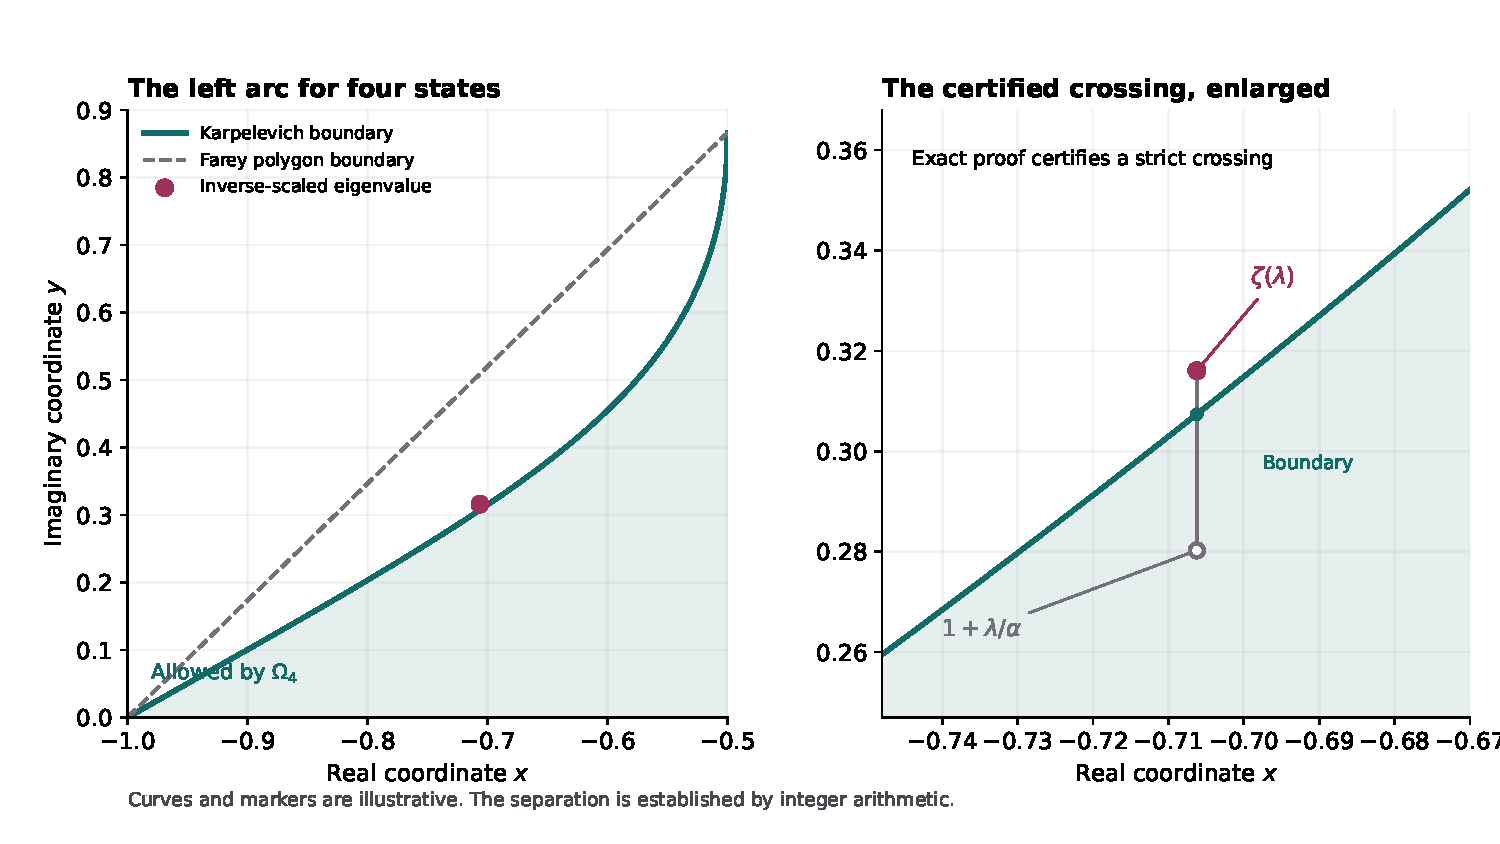
\includegraphics[width=\textwidth]{spectral_geometry.pdf}
\caption{Left: the left boundary arc of \(\Om_4\) (solid) and the edge
of the Farey polygon (dashed). The rescaled eigenvalue of \(\Qw\) lies
outside the arc. Right: magnified view, showing the plain uniformised
point \(1+\lw/\aw\) inside and the rescaled point outside. The
separation is proved by the integer inequality
\eqref{eq:integercertificate}; the figure is illustrative.}
\label{fig:geometry}
\end{figure}

\section{Three states are not enough}
\label{sec:minimal}

\begin{theorem}[Containment in dimensions at most three]
\label{thm:minimal}
Every irreducible bidirectional rate matrix of size \(n\leq3\)
satisfies~\eqref{eq:conjecture}. Hence, within this class, four is the
smallest dimension in which the containment can fail.
\end{theorem}

\begin{proof}
For \(n=1\), \(Q=0\). For \(n=2\) the spectrum is real, and
uniformisation places \(1+\lambda/\alpha\) in \([-1,1]=\Om_2\cap\mathbb
R\); the factor \(\beta\) does not move real points.

Let \(n=3\). Real eigenvalues are handled as before. A nonreal pair
\(a\pm\ii b\) requires \(\beta>0\) (otherwise the spectrum is real), and
the third eigenvalue is zero. Since all escape rates are at most
\(\alpha\), \(2a=\tr Q\geq-3\alpha\), so \(x=1+a/\alpha\ge-\frac12\).
The sector bound conjectured by Barato and Seifert \cite{barato2017}
and proved by Ohga, Ito and Kolchinsky \cite[Eq.~(10)]{ohga2023} states,
for every nonreal eigenvalue of a rate matrix,
\begin{equation}
\frac{|b|}{-a}
\leq\max_c \tanh\frac{|F_c|}{2|c|}\cot\frac{\pi}{|c|},
\label{eq:sector}
\end{equation}
the maximum running over simple cycles with the affinity of
\eqref{eq:affinity}; the bound is invariant under transposition, so the
row/column convention is immaterial. Two-cycles contribute
\(\tanh(0)\cot(\pi/2)=0\). In three states every other simple cycle has
length three, so the right side equals \(\beta\cot(\pi/3)=\beta/\sqrt3\),
and the rescaled coordinate obeys
\begin{equation}
|y|=\frac{|b|}{\alpha\beta}\leq\frac{-a}{\alpha\sqrt3}
=\frac{1-x}{\sqrt3},\qquad -\frac12\leq x\leq1.
\label{eq:triangle}
\end{equation}
This is the triangle with vertices \(1,e^{\pm2\pi\ii/3}\). Every point of
it is an eigenvalue of \(p_0I+p_1C+p_2C^2\), where \(C\) is the cyclic
permutation matrix and \((p_0,p_1,p_2)\) is a probability vector. Hence
the triangle lies in \(\Om_3\).
\end{proof}

\begin{remark}
This concerns containment only. It does not assert that every point of
the affine image is attained for given \((\alpha,\beta)\).
\end{remark}

\section{Where the witness comes from: weak resetting}
\label{sec:family}

\subsection{A boundary matrix}

Choose \(a\in(0,1)\), put
\begin{equation}
t=a^3-a^2+a\in(0,1),
\label{eq:tparam}
\end{equation}
and define
\begin{equation}
P_0(t)=
\begin{pmatrix}
0&1&0&0\\
t&0&1-t&0\\
1-t&0&0&t\\
0&0&1&0
\end{pmatrix}.
\label{eq:P0}
\end{equation}
This is the Johnson--Paparella Type II realising matrix
\(\alpha X+\beta Y\) for the Farey neighbours \(1/3,1/2\) with
\(\beta=t\), \(\alpha=1-t\) \cite[Theorem~3.2]{johnson2017}, after the
relabelling of states \((1,2,3,4)\mapsto(3,4,2,1)\). Its characteristic
polynomial is the boundary polynomial
\begin{equation}
\det(zI-P_0)=(z^2-t)^2-(1-t)^2z,
\label{eq:charP0}
\end{equation}
one root of the cubic factor is \(a^2\), and
\begin{equation}
\spec(P_0)=\{1,a^2,x_0\pm\ii y_0\},
\label{eq:specP0}
\end{equation}
\begin{equation}
x_0=-\frac{1+a^2}{2},\qquad
y_0=\frac{1-a}{2}\sqrt{3a^2-2a+3}>0,\qquad y_0^2=g(x_0).
\label{eq:boundaryparam}
\end{equation}
These follow from the sum and product of the roots.

\subsection{Add resetting that preserves the stationary distribution}

Let \(v=(1,1,1,t)\). Then \(vP_0=v\) and \(v\one=3+t\). For \(\eps>0\) set
\begin{equation}
R_\eps=P_0-I+\eps\{\one v-(3+t)I\}.
\label{eq:Rfamily}
\end{equation}
The added term is resetting at rate \((3+t)\eps\) to the stationary
distribution \(v/(3+t)\). Biochemically, resetting to the stationary
mix is the same as turnover or dilution: a molecule is degraded and
replaced by a fresh one drawn from the steady-state population. The
off-diagonal rates of \(R_\eps\) are
\begin{equation}
\begin{pmatrix}
\cdot&1+\eps&\eps&t\eps\\
t+\eps&\cdot&1-t+\eps&t\eps\\
1-t+\eps&\eps&\cdot&t(1+\eps)\\
\eps&\eps&1+\eps&\cdot
\end{pmatrix},
\label{eq:offdiag}
\end{equation}
all positive; the escape rates are \(1+(2+t)\eps\) (three times) and
\(1+3\eps\), so \(\alpha_\eps=1+3\eps\).

If \(P_0u=zu\) with \(z\ne1\), then \((z-1)vu=0\), so \(vu=0\) and
\(R_\eps u=(z-1-(3+t)\eps)u\). Hence
\begin{equation}
\lambda_\eps=x_0-1-(3+t)\eps+\ii y_0
\label{eq:lambdafamily}
\end{equation}
is an eigenvalue: the uniform shift of \cite{rose2018}. At \(a=2/3\),
\(t=14/27\), \(\eps=1/100\) one has exactly \(\Qw=2700R_{1/100}\), which
explains \eqref{eq:charstar}.

\subsection{The dominant cycle}

Put
\begin{equation}
A_\eps=\frac{1+\eps}{t+\eps}>1,\qquad
B_\eps=\frac{1-t+\eps}{\eps}>1.
\label{eq:AB}
\end{equation}
The seven cycle ratios take the forms of Table~\ref{tab:symbolic}.

\begin{table}[ht]
\centering
\begin{tabular}{@{}lcc@{}}
\toprule
Cycle(s) & Length & Larger forward/backward ratio\\
\midrule
\(123\) & 3 & \(A_\eps B_\eps^2\)\\
\(124\) & 3 & \(A_\eps\)\\
\(134,234\) & 3 & \(B_\eps\)\\
\(1234,1243\) & 4 & \(A_\eps B_\eps\)\\
\(1324\) & 4 & \(B_\eps^2\)\\
\bottomrule
\end{tabular}
\caption{Cycle ratios throughout the resetting family.}
\label{tab:symbolic}
\end{table}

Since \(\log A_\eps,\log B_\eps>0\), the mean
\((\log A_\eps+2\log B_\eps)/3\) exceeds every other mean; for example
its excess over the four-cycle means is
\((\log A_\eps+5\log B_\eps)/12\) and \((2\log A_\eps+\log B_\eps)/6\).
So \(123\) dominates for every \(\eps>0\), and with
\(w_\eps=(A_\eps B_\eps^2)^{-1/3}\),
\begin{equation}
\beta_\eps=\frac{1-w_\eps}{1+w_\eps},\qquad
x_\eps=\frac{x_0-t\eps}{1+3\eps},\qquad
y_\eps=\frac{y_0}{(1+3\eps)\beta_\eps}.
\label{eq:xyfamily}
\end{equation}

\subsection{Two perturbation orders}

\begin{theorem}[Counterexamples near every point of the open arc]
\label{thm:family}
Fix \(a\in(0,1)\) and \(t\) by \eqref{eq:tparam}. Then
\begin{equation}
y_\eps^2-g(x_\eps)
 =4y_0^2\left(\frac{t}{(1-t)^2}\right)^{1/3}\eps^{2/3}
  +O_a(\eps)
\quad(\eps\downarrow0),
\label{eq:asymptoticgap}
\end{equation}
where the implied constant depends on \(a\). Hence there is
\(\eps_0(a)>0\) such that \(R_\eps\) violates \eqref{eq:conjecture} for
all \(0<\eps<\eps_0(a)\).
\end{theorem}

\begin{proof}
From \eqref{eq:AB},
\(w_\eps=(t/(1-t)^2)^{1/3}\eps^{2/3}(1+O(\eps))\), so
\(\beta_\eps^{-2}=1+4(t/(1-t)^2)^{1/3}\eps^{2/3}+O(\eps^{4/3})\). The
factor \((1+3\eps)^{-2}\) changes by \(O(\eps)\), \(x_\eps=x_0+O(\eps)\),
and \(g\) is smooth near the interior point \(x_0\) with
\(g(x_0)=y_0^2\). Subtraction gives \eqref{eq:asymptoticgap}, whose
leading coefficient is positive; since \(\eps=o(\eps^{2/3})\), the gap
is positive for small \(\eps\), and Lemma~\ref{lem:boundary} applies.
\end{proof}

Two edges of the dominant triangle have no reverse transition at
\(\eps=0\). Reverse rates of order \(\eps\) make its ratio grow like
\(\eps^{-2}\); averaging over three edges gives the exponent \(2/3\).
The eigenvalue moves linearly in \(\eps\). As \(\eps\to0\),
\(\beta_\eps\to1\) and the rescaled point returns to the boundary point
\(x_0+\ii y_0\), so the limit itself is not a counterexample.

\section{An explicit interval of counterexamples}
\label{sec:uniform}

Theorem~\ref{thm:family} gives a possibly different neighbourhood of
\(\eps=0\) for each point of the arc. For the witness's parameter we
give one explicit interval.

\begin{theorem}[Uniform interval of counterexamples]
\label{thm:uniform}
Let \(a=2/3\), \(t=14/27\). For every \(0<\eps\leq1/100\),
\begin{equation}
y_\eps^2-g(x_\eps)
\geq\frac{16505}{1527696}\eps^{2/3}>0,
\label{eq:uniformgap}
\end{equation}
so every \(R_\eps\) in this interval violates \eqref{eq:conjecture}.
\end{theorem}

\begin{proof}
Here \(x_0=-13/18\) and \(y_0^2=1/12\). First, \(A_\eps\leq1/t\) and
\(1-t+\eps\leq1327/2700\), so
\[
(A_\eps B_\eps^2)\eps^2
\leq\frac1t\left(\frac{1327}{2700}\right)^2
=\frac{1760929}{3780000}<\frac{64}{125},
\]
hence \(w_\eps\geq(5/4)\eps^{2/3}\). Since \(0<w_\eps<1\),
\(\beta_\eps^{-2}=((1+w_\eps)/(1-w_\eps))^2\geq1+4w_\eps\). Using
\((1+3\eps)^{-2}\geq1-6\eps\) for the baseline term and
\((1+3\eps)^{-2}\geq10000/10609\) for the correction,
\begin{equation}
y_\eps^2
\geq\frac1{12}-\frac\eps2+\frac{12500}{31827}\eps^{2/3}.
\label{eq:heightlower}
\end{equation}
Next, \(0\leq x_\eps-x_0=\frac{89}{54}\frac{\eps}{1+3\eps}
\leq\frac{89}{54}\eps\) and \(x_\eps\in[-13/18,-1964/2781]\). With
\(s=\sqrt{-2x-1}\) one has \(16/25<s\leq2/3\), because
\(\frac{1147}{2781}-(\frac{16}{25})^2=\frac{4939}{1738125}>0\), and
\(g'(x)=-3s^2+6s-5+2/s\). Its derivative in \(s\) is at most
\(54/25-9/2<0\) on this interval, so
\(g'(x)\leq-3(16/25)^2+6(16/25)-5+2/(16/25)=3681/5000<3/4\), and the mean
value theorem gives
\begin{equation}
g(x_\eps)\leq\frac1{12}+\frac{89}{72}\eps.
\label{eq:boundaryupper}
\end{equation}
Therefore
\(y_\eps^2-g(x_\eps)\geq\frac{12500}{31827}\eps^{2/3}-\frac{125}{72}\eps\).
Finally \(\eps^{1/3}<11/50\) because \((11/50)^3=1331/125000>1/100\),
and \(\frac{12500}{31827}-\frac{125}{72}\cdot\frac{11}{50}
=\frac{16505}{1527696}\).
\end{proof}

The constant in \eqref{eq:uniformgap} is conservative; a dense sweep
gives a minimum of \((y_\eps^2-g(x_\eps))/\eps^{2/3}\) near \(0.117\).

\begin{corollary}[An open set of positive-rate counterexamples]
\label{cor:open}
There is an open neighbourhood of \(\Qw\) in \(\mathbb R^{12}\), the
space of off-diagonal rates, consisting of rate matrices that
violate~\eqref{eq:conjecture}.
\end{corollary}

\begin{proof}
The rates of \(\Qw\) are positive, its complex pair is simple,
\(\bw>0\), and \(-1<x<-1/2\). The eigenvalues near this simple pair,
the maximal escape rate, and the maximum of the finitely many cycle
means depend continuously on the rates. Since \(\Om_4\) is closed and
the transformed point lies outside it, it stays outside nearby.
\end{proof}

\section{Five, six and every larger number of states}
\label{sec:all_dimensions}

Appending states to a four-state example does not suffice, because
\(\Om_n\) grows with \(n\). We repeat the construction with the
boundary matrices of each dimension. Throughout, the order of limits
is: fix \(n\); then fix \(t\in(0,\eta_n)\); then let \(\eps\to0\). No
threshold is uniform in \(t\) or in \(n\).

\subsection{Boundary matrices in every dimension}

For even \(n=2m\geq4\) let the nonzero entries of \(P_n(t)\) be
\begin{equation}
P_{2k-1,2k}=1,\ P_{2k,2k-1}=t\ (1\le k\le m),\qquad
P_{2k,2k+1}=1-t\ (1\le k<m),\qquad P_{n,2}=1-t .
\label{eq:even_boundary_matrix}
\end{equation}
For odd \(n=2m+1\geq5\) let them be
\begin{equation}
P_{1,2}=1,\ \ P_{2k,2k+1}=1,\ P_{2k+1,2k}=t\ (1\le k\le m),\ \
P_{2k+1,2k+2}=1-t\ (1\le k<m),\ \ P_{n,1}=1-t .
\label{eq:odd_boundary_matrix}
\end{equation}
These are irreducible stochastic matrices for \(0<t<1\), and direct
expansion gives
\begin{equation}
\det(zI-P_n(t))=F_{n,t}(z):=
\begin{cases}
(z^2-t)^m-(1-t)^m z,&n=2m,\\
z(z^2-t)^m-(1-t)^m,&n=2m+1,
\end{cases}
\label{eq:general_Ito}
\end{equation}
with stationary row vector \(v=(c,1,\ldots,1)\), \(V=v\one=n-1+c\),
where \(c=t\) for even and \(c=1-t\) for odd \(n\).

\begin{lemma}[Which arc]
\label{lem:ito_match}
Let \(s=n-1\) for even \(n\) and \(s=n\) for odd \(n\), and
\(r=(s-1)/2\). Then \(r/s\) and \(1/2\) are Farey neighbours of order
\(n\), and \eqref{eq:ito_general} for this pair, with \(\tau=t\), is
\(F_{n,t}(\lambda)=0\) up to a power of \(\lambda\). The pair is of Johnson--Paparella
Type~II (\(s<2\lfloor n/2\rfloor\)) for even \(n\) and Type~III
(\(s>2\lfloor n/2\rfloor\), \(d=s-2\lfloor n/2\rfloor=1\)) for odd \(n\)
\cite[proof of Theorem~3.2]{johnson2017}, and the characteristic
polynomial of \(P_n(t)\) is the reduced Type~II/III boundary
polynomial. (We do not claim, and nothing below uses, that \(P_n(t)\)
is the Johnson--Paparella realising matrix itself up to a relabelling
of states.)
\end{lemma}

\begin{proof}
\(s\) is odd and \(s\cdot1-2r=1\); since \(s+2>n\), Lemma~\ref{lem:farey}
applies. In \eqref{eq:ito_general} take \(q=2\) (the smaller
denominator) and \(\lfloor n/2\rfloor=m\). For \(n=2m\), \(s=2m-1\):
\(\lambda^{2m-1}(\lambda^2-t)^m=(1-t)^m\lambda^{2m}\), i.e.\
\(\lambda^{2m-1}[(\lambda^2-t)^m-(1-t)^m\lambda]=0\). For \(n=2m+1\),
\(s=2m+1\): \(\lambda^{2m+1}(\lambda^2-t)^m=(1-t)^m\lambda^{2m}\), i.e.\
\(\lambda^{2m}[\lambda(\lambda^2-t)^m-(1-t)^m]=0\). The case
distinction is that of \cite{johnson2017}, where Type~II reads
\((\lambda^q-\beta)^{\lfloor n/q\rfloor}=\alpha^{\lfloor n/q\rfloor}
\lambda^{q\lfloor n/q\rfloor-s}\) and Type~III reads
\(\lambda^d(\lambda^q-\beta)^{\lfloor n/q\rfloor}=\alpha^{\lfloor
n/q\rfloor}\), with \(\beta=t\), \(\alpha=1-t\).
\end{proof}

\begin{lemma}[A smooth boundary point with exterior above]
\label{lem:general_boundary}
Let \(n\ge4\), \(\theta=\pi-\pi/s=2\pi r/s\), \(z_\circ=e^{\ii\theta}\).
There is \(\eta_n>0\) such that for every \(t\in(0,\eta_n)\):
\begin{enumerate}
\item[(i)] the analytic root branch \(z(t)=x(t)+\ii y(t)\) of
\(F_{n,t}\) with \(z(0)=z_\circ\) is a simple eigenvalue of \(P_n(t)\)
and is the point of the boundary arc of \(\Om_n\) from \(z_\circ\) to
\(-1\) at parameter \(\tau=t\);
\item[(ii)] near \(z(t)\), that arc is a smooth graph \(y=h(x)\), and
the points just above the graph lie outside \(\Om_n\).
\end{enumerate}
\end{lemma}

\begin{proof}
\emph{(i) Branch.} At \(t=0\), \(F_{n,0}\) is \(z^{2m}-z=z(z^{s}-1)\)
for even \(n\) and \(z^{2m+1}-1=z^s-1\) for odd \(n\); \(z_\circ\) is a
simple root because \(z_\circ^s=1\) and the derivative there is \(s\),
respectively \(s/z_\circ\). By the implicit function theorem there are
\(\delta,\eta>0\) such that, for \(0\le t<\eta\), \(F_{n,t}\) has exactly
one root in the disc \(|z-z_\circ|<\delta\), namely \(z(t)\). Let
\(\kappa(\tau)\) be the arc point of Theorem~\ref{thm:karp} for this
pair (Lemma~\ref{lem:ito_match}); it is a root of \(F_{n,\tau}\),
depends continuously on \(\tau\) and satisfies \(\kappa(0)=z_\circ\).
Shrinking \(\eta\), \(|\kappa(t)-z_\circ|<\delta\) for \(t<\eta\), so
\(\kappa(t)=z(t)\). Being a root of the characteristic polynomial,
\(z(t)\) is an eigenvalue of \(P_n(t)\), and it is simple for small
\(t\) by continuity.

\emph{Local shape.} Implicit differentiation gives
\begin{equation}
z'(0)=-\frac{2\ii m}{s}\sin\theta,
\qquad
x''(0)=
\begin{cases}
\dfrac{4m(m+1)}{s^2}\cos\theta\sin^2\theta,&n=2m,\\[0.6em]
\dfrac{4m(m-1)}{s^2}\cos\theta\sin^2\theta,&n=2m+1.
\end{cases}
\label{eq:general_derivatives}
\end{equation}
Since \(z'(0)\) is purely imaginary, \(x'(0)=0\); since
\(\cos\theta<0<\sin\theta\) and \(m\ge2\), \(x''(0)<0\) and
\(y'(0)<0\). Hence for small \(t>0\), \(x'(t)<0\), \(y'(t)<0\),
\(y(t)>0\), and the arc near \(z(t)\) is a smooth graph \(y=h(x)\) with
\(h'=y'/x'\). Moreover
\(\frac{d}{dt}\arg z(t)|_{t=0}=-\frac{2m}{s}\cos\theta\sin\theta>0\),
so for small \(t\)
\begin{equation}
x(t)y'(t)-y(t)x'(t)=|z(t)|^2\tfrac{d}{dt}\arg z(t)>0.
\label{eq:transversal}
\end{equation}

\emph{(ii) Exterior side.} Take a small open disc \(D\) around \(z(t)\)
in which the arc is the graph \(y=h(x)\), and which meets no other
arc: other arcs lie in other angular sectors, and the conjugate arc
lies in \(y<0\), while \(z(t)\) is an interior point of the arc with
\(\theta<\arg z(t)<\pi\). Then \(D\setminus\{y=h(x)\}\) consists of two
connected sets \(D_+\) (above) and \(D_-\) (below), neither of which
meets \(\partial\Om_n\); each therefore lies in the interior of
\(\Om_n\) or in its complement. For small \(\delta'>0\), the point
\((1-\delta')z(t)\) belongs to \(\Om_n\) by Lemma~\ref{lem:star}, and
it lies in \(D_-\): to first order,
\((1-\delta')y-h((1-\delta')x)\approx-\delta'(y-h'x)
=-\delta'(yx'-xy')/x'<0\) by \eqref{eq:transversal} and \(x'<0\). So
\(D_-\subseteq\Om_n\). If also \(D_+\subseteq\Om_n\), then
\(D\subseteq\Om_n\) because \(\Om_n\) is closed, and \(z(t)\) would be
an interior point, contradicting \(z(t)\in\partial\Om_n\). Hence
\(D_+\cap\Om_n=\emptyset\).
\end{proof}

\subsection{The leading cycle after completing the support}

Fix \(n\) and \(t\) as in Lemma~\ref{lem:general_boundary}, and let
\begin{equation}
Q_{n,t,\eps}=P_n(t)-I+\eps(\one v-VI),\qquad \eps>0.
\label{eq:general_reset}
\end{equation}
All off-diagonal rates are positive, \(\lambda_\eps=z(t)-1-V\eps\) is an
eigenvalue, and since \(\min_iv_i=c\),
\begin{equation}
\alpha_\eps=1+(n-1)\eps,\qquad
x_\eps=\frac{x(t)-c\eps}{1+(n-1)\eps},\qquad
y_\eps=\frac{y(t)}{[1+(n-1)\eps]\beta_\eps}.
\label{eq:general_coordinates}
\end{equation}

Every simple cycle of the complete graph must be compared. Define
\(d_{ij}=\mathbf 1_{\{P_{ij}>0\}}-\mathbf 1_{\{P_{ji}>0\}}\in\{-1,0,1\}\).
At fixed \(t\),
\begin{equation}
\log\frac{q_{ij}}{q_{ji}}=d_{ij}\log(1/\eps)+b_{ij}+O(\eps),
\label{eq:edge_valuation}
\end{equation}
with finite constants \(b_{ij}\) depending on \(t\).

\begin{lemma}[Unique critical triangle]
\label{lem:critical_triangle}
For each \(P_n(t)\),
\(\max_c|c|^{-1}\bigl|\sum_{(i,j)\in c}d_{ij}\bigr|=2/3\), attained by
exactly one unoriented cycle: \((n,2,3)\) for even \(n\) and
\((n,1,2)\) for odd \(n\).
\end{lemma}

\begin{proof}
The edges with \(d_{ij}=1\) form isolated directed edges and one path
of length two, \(n\to2\to3\) (even) or \(n\to1\to2\) (odd). In an
oriented simple cycle with \(p\) edges of value \(+1\) and \(q\) others,
\(q\ge1\), and the \(+1\) edges form runs of length at most two, so
\(p\le2q\) and the mean is at most \(p/(p+q)\le2/3\); the reverse
orientation is treated in the same way. Equality needs no \(-1\) edges
and all runs of length two; the unique path can be used once, so
\(p=2\), \(q=1\), giving the stated triangle, whose closing edge has
value zero.
\end{proof}

For all sufficiently small \(\eps\) (depending on \(n\) and \(t\)) the
critical triangle therefore has the largest mean affinity, with exact
ratio
\begin{equation}
K_\eps=
\begin{cases}
\dfrac{(1-t+\eps)^2(1+\eps)}{\eps^2(t+\eps)},&n=4,\\[0.7em]
\dfrac{(1-t+\eps)^2}{\eps^2},&n\geq6\text{ even},\\[0.7em]
\dfrac{(1+\eps)^2}{\eps^2},&n\geq5\text{ odd},
\end{cases}
\qquad
w_\eps:=K_\eps^{-1/3}=\kappa_n(t)\eps^{2/3}(1+O(\eps)),
\label{eq:general_triangle_ratio}
\end{equation}
where \(\kappa_4=[t/(1-t)^2]^{1/3}\), \(\kappa_n=(1-t)^{-2/3}\) for even
\(n\ge6\) and \(\kappa_n=1\) for odd \(n\ge5\). For \(n=4\),
\(P_4(t)\) is \(P_0(t)\) of \eqref{eq:P0} after relabelling, and
\(\kappa_4\) agrees with Theorem~\ref{thm:family}.

\begin{theorem}[Failure in every dimension at least four]
\label{thm:all_dimensions}
For every \(n\geq4\) there is \(\eta_n>0\) such that for each fixed
\(t\in(0,\eta_n)\) there is \(\eps_0(n,t)>0\) with the following
property: for \(0<\eps<\eps_0(n,t)\), \(Q_{n,t,\eps}\) violates
\eqref{eq:conjecture}, and so does every rate matrix in an open
neighbourhood of it in \(\mathbb R^{n(n-1)}\). Together with
Theorem~\ref{thm:minimal}, universal containment over irreducible
bidirectional rate matrices holds exactly in dimensions \(n\le3\).
\end{theorem}

\begin{proof}
By \eqref{eq:general_triangle_ratio},
\(\beta_\eps^{-1}=(1+w_\eps)/(1-w_\eps)=1+2\kappa_n\eps^{2/3}+O(\eps^{4/3})\),
so \eqref{eq:general_coordinates} gives \(x_\eps=x(t)+O(\eps)\) and
\(y_\eps=y(t)+2y(t)\kappa_n\eps^{2/3}+O(\eps)\). Since \(h\) is smooth
near \(x(t)\), \(h(x_\eps)=y(t)+O(\eps)\), and
\begin{equation}
y_\eps-h(x_\eps)=2y(t)\kappa_n(t)\eps^{2/3}+O_{n,t}(\eps)>0
\label{eq:all_dimensional_gap}
\end{equation}
for small \(\eps\). By Lemma~\ref{lem:general_boundary}(ii) the rescaled
eigenvalue lies outside \(\Om_n\). The eigenvalue is simple, the rates
are positive and the separation strict, so the continuity argument of
Corollary~\ref{cor:open} gives an open set.
\end{proof}

For \(n=3\) the odd formula in \eqref{eq:general_derivatives} has
\(m=1\) and gives \(x''(0)=0\): the pair stays on the line
\(x=-1/2\), the upward-exterior geometry is absent, in agreement with
Theorem~\ref{thm:minimal}.

\subsection{How small must \texorpdfstring{\(\eps\)}{epsilon} be?}

\begin{remark}[The \(\eps\)-scale]
\label{rem:scale}
The remainder in \eqref{eq:all_dimensional_gap} hides constants that
depend strongly on \(t\), for two reasons. First, the constants
\(b_{ij}\) in \eqref{eq:edge_valuation} contain \(\log(1/t)\), so a
long cycle with smaller valuation mean can beat the critical triangle
until \(\eps\) is very small. In five states the competitor is the
Hamiltonian cycle \(1\to2\to3\to4\to5\to1\), whose ratio behaves like
\(\eps^{-3}t^{-2}\): its mean affinity
\(\frac35\log\frac1\eps+\frac25\log\frac1t\) falls below the triangle's
\(\frac23\log\frac1\eps\) only when, up to bounded factors,
\(\eps\lesssim t^{6}\) (more precisely
\(\eps\lesssim t^6/(1-t)^3\)). Second, near the arc endpoint the local
boundary slope is of order \(1/t\), so the \(O(\eps)\) term carries a
factor of order \(1/t\), and positivity of \eqref{eq:all_dimensional_gap}
needs roughly \(\eps^{1/3}\ll t\). For the proof's asymptotics the first condition
dominates. Numerically, at \(t=1/20\) the five-, six- and
seven-state gaps are still negative at \(\eps=10^{-6}\). In five states
the triangle becomes dominant near \(\eps\approx e^{-18}\approx t^6\),
and the radial margin is already positive from about
\(\eps\approx e^{-16.3}\); \(\eps\lesssim t^6\) is what the proof's
asymptotics need, not a threshold for violation. The small-\(t\)
hypothesis is a convenience of the proof: at moderate \(t\) (e.g.\
\(t\approx0.3\)--\(0.6\)) violations appear already for
\(\eps\approx10^{-5}\)--\(10^{-4}\), which is how the certified
instances below were chosen. Violations in dimension \(n\ge5\) are
real but thin: margins are of order \(10^{-4}\) or smaller.
\end{remark}

\subsection{Exactly certified counterexamples in five and six states}
\label{sec:certified}

\begin{theorem}[Certified instances]
\label{thm:certified}
The rate matrices \(Q_{5,3/5,1/40000}\) and \(Q_{6,1/2,1/8000}\) of
\eqref{eq:general_reset} have rational entries and positive
off-diagonal rates, and both violate \eqref{eq:conjecture}.
\end{theorem}

\begin{proof}[Proof (computer-assisted, exact)]
The script \path{certify_higher_dimensions.py} uses only integers,
rational numbers and outward-rounded rational interval arithmetic
(fixed-point grid \(2^{-128}\)); no floating-point value enters any
decision. For each instance it verifies:
\begin{enumerate}
\item row sums, positivity, \(\alpha=1+(n-1)\eps\), \(vP_n=v\),
\(\det(zI-P_n(t))=F_{n,t}(z)\) and
\(\det(zI-Q)=z\,G(z+1+V\eps)\) with \(G=F_{n,t}/(z-1)\), all as exact
polynomial identities;
\item a rational disc of radius below \(10^{-27}\) containing a root
\(z^*\) of \(F_{n,t}\) with \(\operatorname{Im}z^*>0\), \(z^*\ne1\), by
the classical bound that some root of a polynomial \(p\) of degree
\(d\) lies within \(d|p(z_0)|/|p'(z_0)|\) of \(z_0\) (evaluated
exactly); thus \(\lambda=z^*-1-V\eps\) is an eigenvalue of \(Q\);
\item the exact ratio of every simple cycle of the complete graph
(\(37\) unoriented cycles for \(n=5\), \(197\) for \(n=6\)), the
dominant cycle by exact comparison \(K_c^{|d|}\) versus \(K_d^{|c|}\),
and rational bounds \(\beta_{\rm lo}\le\beta\le\beta_{\rm hi}\);
\item a rational box \(W\) of width below \(10^{-37}\) containing the
rescaled eigenvalue;
\item a rational \(S\) with \(S^2\min_{w\in W}|w|^2\ge1\), and the
hypothesis of Lemma~\ref{lem:exterior_test} for \(W\), for all Farey
pairs of order \(n\): \([1,S]\times[0,1]\) is bisected into closed
boxes, and on each terminal box the interval extension of
\((\sigma w)^s\bigl((\sigma w)^q-\tau\bigr)^k-(1-\tau)^k(\sigma w)^{qk}\),
\(k=\lfloor n/q\rfloor\), obtained by evaluating this expression in
rectangular complex interval arithmetic with powers by binary
(square-and-multiply) powering, has a real or an imaginary part that
excludes~\(0\).
\end{enumerate}
Lemma~\ref{lem:exterior_test} then gives \(W\cap\Om_n=\emptyset\).
The terminal boxes are written to \path{exterior_certificates.json}.
A separate checker, \path{check_exterior_certificate.py}, shares no
code with the certifier and uses exact rational intervals without
rounding. It recomputes items 1--5 from \(Q\) and the certificate: the
characteristic polynomial of \(Q\) itself, the cycle ratios, the root
bound, the inclusion of the image of the root disc in \(W\), the bound
on \(S\), and, for every Farey pair, that the boxes are inside
\([1,S]\times[0,1]\), pairwise interior-disjoint and of total area
\(S-1\) (so, being closed, they cover the rectangle), and that each
box excludes~\(0\). Appendix~\ref{app:certificates} prints the data.
\end{proof}

Table~\ref{tab:certified} summarises the receipts. As a control, the
same exterior test certifies the four-state witness \(\Qw\)
independently of Lemma~\ref{lem:boundary}, and fails, as it should,
for points \(10^{-6}\) below the left arc of \(\Om_4\).

\begin{table}[htbp]
\centering
\small
\begin{tabular}{@{}cccccc@{}}
\toprule
\(n\) & \(t\) & \(\eps\) & dominant cycle & rescaled eigenvalue \(\zeta\) & radial margin\\
\midrule
4 & \(14/27\) & \(1/100\) & \((1,2,3)\) & \(-0.706221+0.316083\,\ii\) & \(\approx8.7\times10^{-3}\)\textsuperscript{a}\\
5 & \(3/5\) & \(1/40000\) & \((1,2,5)\) & \(-0.849362+0.248186\,\ii\) & \(\approx4.7\times10^{-5}\)\\
6 & \(1/2\) & \(1/8000\) & \((2,3,6)\) & \(-0.874426+0.253551\,\ii\) & \(\approx2.2\times10^{-4}\)\\
\bottomrule
\end{tabular}
\caption{Certified counterexamples. The radial margin is the
difference between \(|\zeta|\) and the modulus of the boundary point on
the same ray, computed numerically for scale only (\textsuperscript{a}for \(n=4\) the vertical excess over the arc is shown). In five and six
states the runner-up cycle is a Hamiltonian cycle (respectively the
five-cycle \(2\to3\to4\to5\to6\)), in line with
Remark~\ref{rem:scale}.}
\label{tab:certified}
\end{table}

\section{Consequences and open problems}
\label{sec:discussion}

\subsection{The valid bounds and the size of the error}

Because \(\Om_n\) lies in the unit disc, the false containment
\eqref{eq:conjecture} would imply the affinity ellipse, but not
conversely; \(\Qw\) separates the two. The polygon bound of
\cite[Theorem~5]{kolchinsky2026} places the rescaled spectrum in the
convex hull of the roots of unity of order at most \(n\); this polygon
contains \(\Om_n\), and Kolchinsky et al.\ note that it is weaker than
the Karpelevich region in the irreversible limit. Our example is
consistent with it, and checkable without decimals: the ratio of cycle
\(123\) exceeds \(9^3\), so \(\bw>4/5\), and
\[
1-x^2-\frac{607500}{2781^2(4/5)^2}=\frac{11709785}{30935844}>0
\]
gives \(x^2+y^2<1\); at this \(x\) the polygon edge is
\(y=(1+x)\sqrt3\), and \(450/\bw<1125/2<817\) with \(1+x=817/2781\)
puts the point below it. The refinements of \cite{xu2026} concern
unicyclic networks and do not apply to our construction.

If \eqref{eq:conjecture} were used to infer an affinity from
\(\lw\), it would demand
\[
\beta\geq\frac{450\sqrt3/2781}{\sqrt{g(-1964/2781)}}\approx0.9117,
\]
that is \(M=2\operatorname{arctanh}\beta\approx3.075\), whereas
\(M(\Qw)=\frac13\log(177853829/38529)\approx2.812\): an overestimate of
about \(9.3\%\). The error is bounded by the gap between \(\Om_n\) and
the proved polygon, so it is modest, but it is in the unsafe direction.
We know of no empirical study that has used the conjectured region in
this way.

\subsection{Relation to other spectral regions for generators}

Chru\'sci\'nski, Denisov, Tarnowski and \.Zyczkowski
\cite{chruscinski2025} propose a rescaling of classical generators under
which the eigenvalues lie in modified Karpelevi\v{c} regions. As
described there, that rescaling involves no cycle-affinity parameter;
our results concern only the affinity flattening by \(\beta'\), and
neither statement implies the other. Verbeken and Ginis
\cite{verbeken2026} determine the spectral region of stochastic
matrices supported on a directed \(n\)-cycle with self-loops, which
arise from uniformised unidirectional reaction cycles; this is the
irreversible single-cycle analogue of the open problem below.

\subsection{Open problems}

\begin{problem}[Single-cycle networks]
\label{prob:unicyclic}
Does \eqref{eq:conjecture} hold for every rate matrix whose support is a
single bidirectional cycle?
\end{problem}

This is the setting in which (S3) was tested \cite{xu2025}, and our
mechanism does not apply to it: a ring has only one cycle, so weak
reverse rates on some edges cannot create a separate, more strongly
driven triangle. For uniform rings the rescaled eigenvalues are exactly
the \(n\)-th roots of unity, on \(\partial\Om_n\). A multistart local
search over all forward and backward rates of rings with four and five
states (400 starts each, measuring the largest radial excess of any
rescaled eigenvalue over a tabulated boundary of \(\Om_n\)) found no
violation; the largest values, \(-7\times10^{-5}\) and
\(-3\times10^{-4}\), are at the resolution of the tabulation and occur
near uniform rings. This is evidence, not proof, and we make no claim
either way.

\begin{problem}[The true region]
Determine the exact eigenvalue region for given \(n\), \(\alpha\) and
\(\beta\), or at least the largest radial excess over \(\Om_n\) as a
function of \(\beta\). Is the affine containment asymptotically correct
near equilibrium (\(\beta\to0\))? Does a different affinity statistic,
for example one weighted by stationary flux, restore a Karpelevich-shaped
bound? Does containment hold over each fixed sparse topology, such as a
ring with one chord?
\end{problem}

\begin{problem}[Other arcs and explicit thresholds]
Give explicit \(\eta_n\) and \(\eps_0(n,t)\) in
Theorem~\ref{thm:all_dimensions}, and decide whether the resetting
mechanism breaks containment near every arc of \(\Om_n\) whose
realising matrix has one-way edges, not only the arc ending at \(-1\).
\end{problem}

\section*{Declarations}
\addcontentsline{toc}{section}{Declarations}

\paragraph{Data and code availability.} The accompanying bundle, archived at \url{https://doi.org/10.5281/zenodo.23687327} and available at \url{https://github.com/ipitchford/affinity-karpelevich-threshold} (tag \texttt{v1.0.0-candidate}),
contains the exact verifiers \path{verify_affine_counterexample.py}
(four-state witness), \path{audit_karpelevich.py},
\path{audit_all_dimensions.py}, \path{extension_fingerprint.py}
(exact fingerprints of the constructions for \(n=4,5,6\) at
\(t=1/2\), \(\eps=1/1000\); these identify the matrices and the
critical triangle but do not test separation),
\path{certify_higher_dimensions.py} (Theorem~\ref{thm:certified};
it also writes the terminal boxes to \path{exterior_certificates.json}),
the separate checker \path{check_exterior_certificate.py}, and
\path{plot_geometry.py} (figures; illustration only). Each script
writes its receipt to an output directory given by \texttt{--out}
(default \path{receipts/}) and refuses to overwrite existing files.
All scripts were rerun from a clean copy with Python 3.11.14
(\texttt{uv run python3 -I}); the verifiers use only the standard
library, and the figure script uses NumPy and Matplotlib. Decimal
fields in receipts are for orientation and may differ in the last
digits between platforms; all decisive fields are exact.

\paragraph{Literature search.} We searched arXiv and the published
literature to 27 October 2026 for refutations or restatements of the
affine Karpelevich conjecture, including the follow-up works
\cite{kolchinsky2026,xu2026,verbeken2026,chruscinski2025}. None
contains a counterexample or discusses the conjecture's failure;
\cite{kolchinsky2026} remarks only that its polygon bound is weaker than
the Karpelevich region in the irreversible limit. This is a bounded
search, not a priority claim.

\paragraph{Use of AI tools.} The research, the computer-assisted
certificates, the manuscript text and this revision were produced with
the assistance of AI language-model tools, operating under human
direction. The tools were used to search the literature, derive and
check proofs, write and run the verification scripts, and draft and
edit the text. All mathematical claims are supported either by the
proofs in the paper or by the exact-arithmetic scripts in the bundle,
which can be rerun independently.

\paragraph{Competing interests and funding.} None.

\appendix
\section{Certificate data for the five- and six-state instances}
\label{app:certificates}

This appendix prints the data behind Theorem~\ref{thm:certified}, so that
the certificate can be checked from the paper and the receipt
\path{receipts/higher_dimension_certificates.json}. The terminal boxes
(\(352\) for \(n=5\), \(578\) for \(n=6\)) are in
\path{receipts/exterior_certificates.json}; they are too many to print,
and \path{check_exterior_certificate.py} checks them. All numbers below
are exact unless marked with a decimal point. Decimal margins are for
orientation only and play no part in the proof.

\subsection{\texorpdfstring{\(n=5\), \(t=3/5\), \(\eps=1/40000\)}{n=5}}

\paragraph{Rate matrix.} Rows sum to zero and \(\alpha=\tfrac{10001}{10000}\):
{\small\[Q=\frac{1}{200000}\begin{pmatrix}-200020&200005&5&5&5\\
2&-200017&200005&5&5\\
2&120005&-200017&80005&5\\
2&5&5&-200017&200005\\
80002&5&5&120005&-200017\end{pmatrix}.\]}
\paragraph{Cycles.} The complete graph on 5 states has 37 unoriented simple cycles. The ratio of a cycle \(c\) is \(K_c=\prod_{(i\to j)\in c}Q_{ij}/Q_{ji}\), oriented so that \(K_c\ge1\); its mean affinity is \(\frac1{|c|}\log K_c\).
\begin{itemize}
\item Dominant: \((1,2,5)\), \(K=1600080001\), mean affinity \(7.06443982\).
\item Runner-up: \((1,2,3,4,5)\), \(K=\tfrac{40966656409612160176001}{576048001}\), mean affinity \(6.37906877\).
\end{itemize}
The dominance is checked exactly by \(K_c^{|d|}>K_d^{|c|}\). Hence \(\beta=(K^{1/3}-1)/(K^{1/3}+1)\) with the dominant \(K\); the certificate uses rational bounds with \(\beta\in[\beta_{\rm lo},\beta_{\rm hi}]\), \(\beta\approx0.998291513263596\).

\paragraph{Eigenvalue enclosure.} A root \(z^*\) of \(F_{5,t}\) lies within \(R=2\cdot10^{-60}\) of
a centre \(z_0\) with
\begin{align*}
\operatorname{Re}z_0&=-1364992729783575580602216136754888815555776909580718988082285\cdot2^{-200},\\
\operatorname{Im}z_0&=398178175056774674863057881878734891570990524557825817951957\cdot2^{-200},
\end{align*}
so \(\lambda=z^*-1-V\eps\) is an eigenvalue of \(Q\). The rescaled eigenvalue \(\zeta\approx-0.849362124948763+0.248186133174560\,\ii\) lies in the box \(W=[x_{\rm lo},x_{\rm hi}]\times[y_{\rm lo},y_{\rm hi}]\) with
\begin{align*}
x_{\rm lo}&=-289022954250562855660191002779311025953\cdot2^{-128},\\ x_{\rm hi}&=-72255738562640713915047750694827756487\cdot2^{-126},\\
y_{\rm lo}&=21113341208398638187405553346515067939\cdot2^{-126},\\ y_{\rm hi}&=42226682416797276374811106693030135879\cdot2^{-127},
\end{align*}
of width below \(1.469\times10^{-38}\), and \(S=\tfrac{28252422707997040717}{25000000000000000000}\) satisfies \(S^2\min_W|w|^2\ge1\).

\paragraph{Farey and arc tests.} For each Farey pair the bisection of \([1,S]\times[0,1]\) visits the listed number of boxes; the terminal boxes cover the rectangle, and on each one the interval extension excludes 0. The last column is the smallest distance from 0 of the excluding real or imaginary enclosure over the terminal boxes. The tightest pairs are \(2/5,1/2\) and its reflection \(1/2,3/5\): the eigenvalue lies just outside the arc between \(e^{4\pi\ii/5}\) and \(-1\). The radial margin, the distance between \(|\zeta|\) and the outermost boundary point on its ray, is \(\approx4.669\times10^{-5}\) (floating point, for scale only).
\begin{center}\small
\begin{tabular}{@{}lcccrrr@{}}
\toprule
pair & \(q\) & \(s\) & \(k\) & visited & terminal & min.\ margin\\
\midrule
\(0,1/5\) & 1 & 5 & 5 & 25 & 13 & \(1.82\times10^{-2}\)\\
\(1/5,1/4\) & 4 & 5 & 1 & 7 & 4 & \(2.57\times10^{-2}\)\\
\(1/4,1/3\) & 3 & 4 & 1 & 7 & 4 & \(7.26\times10^{-2}\)\\
\(1/3,2/5\) & 3 & 5 & 1 & 1 & 1 & \(7.64\times10^{-2}\)\\
\(2/5,1/2\) & 2 & 5 & 2 & 307 & 154 & \(8.78\times10^{-7}\)\\
\(1/2,3/5\) & 2 & 5 & 2 & 307 & 154 & \(8.78\times10^{-7}\)\\
\(3/5,2/3\) & 3 & 5 & 1 & 1 & 1 & \(7.64\times10^{-2}\)\\
\(2/3,3/4\) & 3 & 4 & 1 & 7 & 4 & \(7.26\times10^{-2}\)\\
\(3/4,4/5\) & 4 & 5 & 1 & 7 & 4 & \(2.57\times10^{-2}\)\\
\(4/5,1\) & 1 & 5 & 5 & 25 & 13 & \(1.82\times10^{-2}\)\\
\bottomrule
\end{tabular}
\end{center}

\subsection{\texorpdfstring{\(n=6\), \(t=1/2\), \(\eps=1/8000\)}{n=6}}

\paragraph{Rate matrix.} Rows sum to zero and \(\alpha=\tfrac{1601}{1600}\):
{\small\[Q=\frac{1}{16000}\begin{pmatrix}-16010&16002&2&2&2&2\\
8001&-16009&8002&2&2&2\\
1&2&-16009&16002&2&2\\
1&2&8002&-16009&8002&2\\
1&2&2&2&-16009&16002\\
1&8002&2&2&8002&-16009\end{pmatrix}.\]}
\paragraph{Cycles.} The complete graph on 6 states has 197 unoriented simple cycles. The ratio of a cycle \(c\) is \(K_c=\prod_{(i\to j)\in c}Q_{ij}/Q_{ji}\), oriented so that \(K_c\ge1\); its mean affinity is \(\frac1{|c|}\log K_c\).
\begin{itemize}
\item Dominant: \((2,3,6)\), \(K=16008001\), mean affinity \(5.52953307\).
\item Runner-up: \((2,3,4,5,6)\), \(K=256128020001\), mean affinity \(5.25378864\).
\end{itemize}
The dominance is checked exactly by \(K_c^{|d|}>K_d^{|c|}\). Hence \(\beta=(K^{1/3}-1)/(K^{1/3}+1)\) with the dominant \(K\); the certificate uses rational bounds with \(\beta\in[\beta_{\rm lo},\beta_{\rm hi}]\), \(\beta\approx0.992095680385056\).

\paragraph{Eigenvalue enclosure.} A root \(z^*\) of \(F_{6,t}\) lies within \(R=2\cdot10^{-60}\) of
a centre \(z_0\) with
\begin{align*}
\operatorname{Re}z_0&=-1405925988550798938004119301164136760896295741542989741518381\cdot2^{-200},\\
\operatorname{Im}z_0&=202236283987962942996587631290827571140088949282185834032295\cdot2^{-199},
\end{align*}
so \(\lambda=z^*-1-V\eps\) is an eigenvalue of \(Q\). The rescaled eigenvalue \(\zeta\approx-0.874425874457829+0.253550827099820\,\ii\) lies in the box \(W=[x_{\rm lo},x_{\rm hi}]\times[y_{\rm lo},y_{\rm hi}]\) with
\begin{align*}
x_{\rm lo}&=-297551706257421405089668952259855843307\cdot2^{-128},\\ x_{\rm hi}&=-148775853128710702544834476129927921651\cdot2^{-127},\\
y_{\rm lo}&=21569718895072058098458530798288771361\cdot2^{-126},\\ y_{\rm hi}&=43139437790144116196917061596577542723\cdot2^{-127},
\end{align*}
of width below \(1.469\times10^{-38}\), and \(S=\tfrac{6864780988993527561}{6250000000000000000}\) satisfies \(S^2\min_W|w|^2\ge1\).

\paragraph{Farey and arc tests.} For each Farey pair the bisection of \([1,S]\times[0,1]\) visits the listed number of boxes; the terminal boxes cover the rectangle, and on each one the interval extension excludes 0. The last column is the smallest distance from 0 of the excluding real or imaginary enclosure over the terminal boxes. The tightest pairs are \(2/5,1/2\) and its reflection \(1/2,3/5\): the eigenvalue lies just outside the arc between \(e^{4\pi\ii/5}\) and \(-1\). The radial margin, the distance between \(|\zeta|\) and the outermost boundary point on its ray, is \(\approx2.210\times10^{-4}\) (floating point, for scale only).
\begin{center}\small
\begin{tabular}{@{}lcccrrr@{}}
\toprule
pair & \(q\) & \(s\) & \(k\) & visited & terminal & min.\ margin\\
\midrule
\(0,1/6\) & 1 & 6 & 6 & 19 & 10 & \(3.21\times10^{-2}\)\\
\(1/6,1/5\) & 5 & 6 & 1 & 3 & 2 & \(2.67\times10^{-1}\)\\
\(1/5,1/4\) & 4 & 5 & 1 & 7 & 4 & \(1.08\times10^{-1}\)\\
\(1/4,1/3\) & 3 & 4 & 2 & 15 & 8 & \(2.13\times10^{-2}\)\\
\(1/3,2/5\) & 3 & 5 & 2 & 7 & 4 & \(8.34\times10^{-2}\)\\
\(2/5,1/2\) & 2 & 5 & 3 & 521 & 261 & \(4.43\times10^{-6}\)\\
\(1/2,3/5\) & 2 & 5 & 3 & 521 & 261 & \(4.43\times10^{-6}\)\\
\(3/5,2/3\) & 3 & 5 & 2 & 7 & 4 & \(8.34\times10^{-2}\)\\
\(2/3,3/4\) & 3 & 4 & 2 & 15 & 8 & \(2.13\times10^{-2}\)\\
\(3/4,4/5\) & 4 & 5 & 1 & 7 & 4 & \(1.08\times10^{-1}\)\\
\(4/5,5/6\) & 5 & 6 & 1 & 3 & 2 & \(2.67\times10^{-1}\)\\
\(5/6,1\) & 1 & 6 & 6 & 19 & 10 & \(3.21\times10^{-2}\)\\
\bottomrule
\end{tabular}
\end{center}


\begin{thebibliography}{99}

\bibitem{barato2017}
Barato, A.~C., \& Seifert, U. (2017).
Coherence of biochemical oscillations is bounded by driving force and
network topology.
\emph{Physical Review E, 95}, 062409.
\url{https://doi.org/10.1103/PhysRevE.95.062409}.

\bibitem{chruscinski2025}
Chru\'sci\'nski, D., Denisov, S., Tarnowski, W., \& \.Zyczkowski, K.
(2025).
\emph{Spectral delineation of Markov generators: classical vs quantum}.
arXiv:2504.07903.
\url{https://doi.org/10.48550/arXiv.2504.07903}.

\bibitem{ito1997}
Ito, H. (1997).
A new statement about the theorem determining the region of eigenvalues
of stochastic matrices.
\emph{Linear Algebra and its Applications, 267}, 241--246.
\url{https://doi.org/10.1016/S0024-3795(97)00018-9}.

\bibitem{johnson2017}
Johnson, C.~R., \& Paparella, P. (2017).
A matricial view of the Karpelevi\v{c} theorem.
\emph{Linear Algebra and its Applications, 520}, 1--15.
\url{https://doi.org/10.1016/j.laa.2017.01.009}.

\bibitem{karpelevich1951}
Karpelevi\v{c}, F.~I. (1951).
On the characteristic roots of matrices with nonnegative elements.
\emph{Izvestiya Akademii Nauk SSSR, Seriya Matematicheskaya, 15},
361--383. English translation: \emph{American Mathematical Society
Translations, Series~2, 140} (1988), 79--100.
\url{https://doi.org/10.1090/trans2/140/05}.

\bibitem{kirkland2022}
Kirkland, S., \& \v{S}migoc, H. (2022).
Stochastic matrices realising the boundary of the Karpelevi\v{c} region.
\emph{Linear Algebra and its Applications, 635}, 116--138.
\url{https://doi.org/10.1016/j.laa.2021.11.016}.

\bibitem{kolchinsky2026}
Kolchinsky, A., Ohga, N., \& Ito, S. (2026).
\emph{Cycle affinity and winding localize eigenvalues of Markov
generators} (Version 3, 8 October 2026). arXiv:2605.15884.
\url{https://doi.org/10.48550/arXiv.2605.15884}.

\bibitem{ohga2023}
Ohga, N., Ito, S., \& Kolchinsky, A. (2023).
Thermodynamic bound on the asymmetry of cross-correlations.
\emph{Physical Review Letters, 131}, 077101.
\url{https://doi.org/10.1103/PhysRevLett.131.077101}.

\bibitem{rose2018}
Rose, D.~C., Touchette, H., Lesanovsky, I., \& Garrahan, J.~P. (2018).
Spectral properties of simple classical and quantum reset processes.
\emph{Physical Review E, 98}, 022129.
\url{https://doi.org/10.1103/PhysRevE.98.022129}.

\bibitem{uhl2019}
Uhl, M., \& Seifert, U. (2019).
Affinity-dependent bound on the spectrum of stochastic matrices.
\emph{Journal of Physics A: Mathematical and Theoretical, 52}, 405002.
\url{https://doi.org/10.1088/1751-8121/ab3a7a}.

\bibitem{verbeken2026}
Verbeken, B.~F., \& Ginis, V. (2026).
\emph{On the spectral region of \(n\)-cycle stochastic matrices}
(Version 2, 14 September 2026). arXiv:2606.10143.
\url{https://doi.org/10.48550/arXiv.2606.10143}.

\bibitem{xu2025}
Xu, G.-H., Kolchinsky, A., Delvenne, J.-C., \& Ito, S. (2025).
Thermodynamic geometric constraint on the spectrum of Markov rate
matrices.
\emph{Physical Review Letters, 135}, 257102.
\url{https://doi.org/10.1103/z4t2-18cx}.
Supplement inspected at \url{https://arxiv.org/abs/2507.08938v2}.

\bibitem{xu2026}
Xu, R., \& Meng, C. (2026).
\emph{Kinetic heterogeneity tightens thermodynamic bounds on spectra of
Markov cycles} (Version 2, 3 October 2026). arXiv:2608.22934.
\url{https://doi.org/10.48550/arXiv.2608.22934}.

\end{thebibliography}
\end{document}
